 
\documentclass[crop,border={0pt 0 0 0},tikz]{standalone}
\usetikzlibrary{backgrounds,decorations.markings}
\tikzset{>=latex}
\tikzset{->-/.style={decoration={
  markings,
  mark=at position .5 with {\arrow{>}}},postaction={decorate}}}
\begin{document}
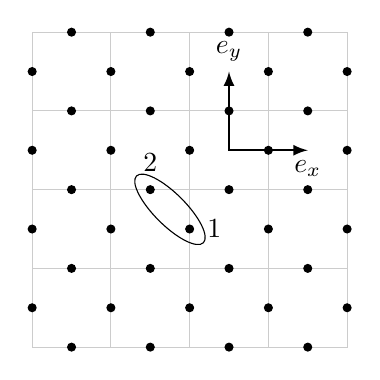
\begin{tikzpicture}
    
    \draw [step=1, line cap = rect, gray!40] (0,0) grid (4,4);
    
    \foreach \i in {0,...,3}
    { 
        \foreach \j in {0,...,3}
        {
            \draw[fill, xshift=0.5cm, yshift=0.5cm] (\i+0.5,\j) circle [radius=0.05];
            \draw[fill, xshift=0.5cm, yshift=0.5cm] (\i,\j+0.5) circle [radius=0.05];

        }
        
        \draw[fill, xshift=0.5cm, yshift=0.5cm] (-0.5,\i) circle [radius=0.05];
        \draw[fill, xshift=0.5cm, yshift=0.5cm] (\i,-0.5) circle [radius=0.05];
    }

    \draw[black, rotate around={-45:(1.75,1.75)}] (1.75,1.75) ellipse (0.6 and 0.2);
    \node[anchor=south] at (1.5,2.1) {$2$};
    \node[anchor=west] at (2.1,1.5) {$1$};

    \draw [thick,->] (2.5,2.5) -- +(1,0) node[anchor=north]{$e_x$};
    \draw [thick,->, line cap=rect] (2.5,2.5) -- +(0,1) node[anchor=south]{$e_y$};

\end{tikzpicture}
\end{document}
